\documentclass[10pt,aspectratio=169]{beamer}

\usetheme{Frankfurt}

\usepackage[utf8]{inputenc}

\title{Shimmer code architecture proposal}
\author{Matteo Cicuttin}
\institute{DISMA - PoliTO}

\begin{document}
\maketitle

\begin{frame}{Objectives}
    Simulate a gas distribution network:
    \begin{itemize}
        \item Stations are nodes
        \item Interconnections are edges
        \item Both nodes and edges have properties
    \end{itemize}

    Gas flow is governed by some mathematical model
\end{frame}

\begin{frame}{System boundaries}
    \begin{itemize}
        \item On-disk network representation \& data interchange
        \item In-memory network representation
        \item Numerical models
    \end{itemize}
\end{frame}

\begin{frame}{Data exchange and on-disk representation}
    \begin{itemize}
        \item Gas network data should be easily exchanged
        \item Data format should guarantee data correctness
    \end{itemize}

    Natural choiche: SQLite

    \begin{itemize}
        \item Full fledged SQL database, data constraints easily specified \& enforced
        \item Wide support on all main OSs, Matlab supports it natively
        \item Graphical tools for data manipulation \& import/export
    \end{itemize}
\end{frame}

\begin{frame}{Oversimplified relational data model}
    \begin{minipage}{0.6\textwidth}
        \begin{center}
            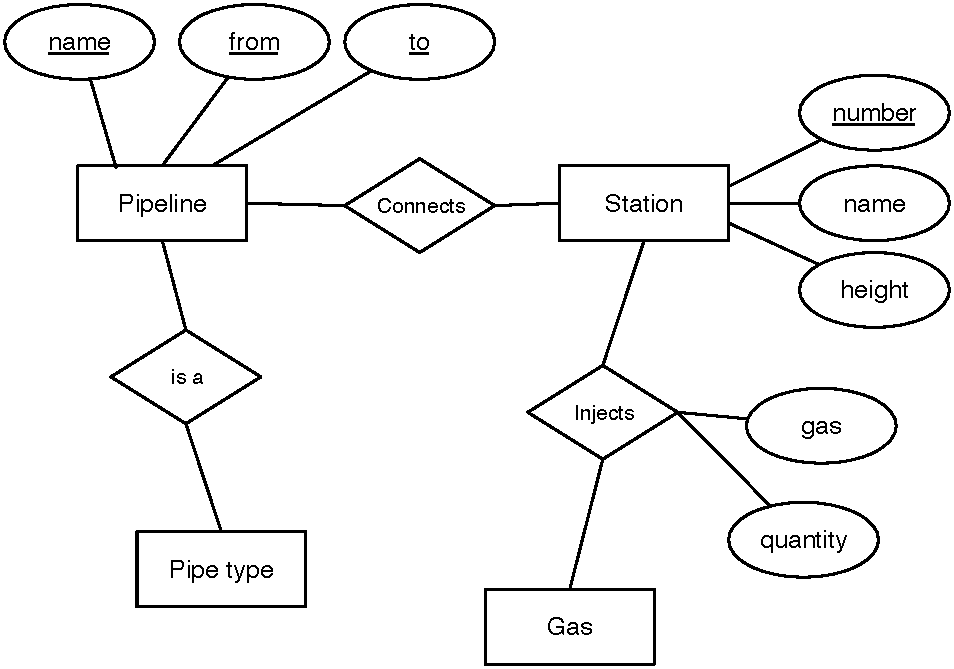
\includegraphics[width=0.9\textwidth]{img/data_arch}
        \end{center}
    \end{minipage}
    \begin{minipage}{0.39\textwidth}
        Relational data models are ubiquitous and well-understood:
        \begin{itemize}
            \item Clear and unambiguous \textbf{entities} and \textbf{relations}
            \item Data integrity automatically checked: impossible to enter an edge if a node does not exist
        \end{itemize}
    \end{minipage}
\end{frame}

\end{document}
